\chapter{函数与极限}
\section{利用定义证明极限}
\subsection{自变量趋于有限值时函数的极限}
\tdefination[函数极限1]
设函数$f(x)$在点$x_0$的某一去心邻域\index{QXLY@去心领域}\footnote{去心邻域指的是以$x_0$为中心的连续区间$U(x_0)$去掉中心$x_0$后的新区间,记为$U\degree (x_0 )$.特别注意的是,去心邻域仅在中心$x_0$处没有定义,其它点都有定义.}内有定义.如果存在常数$A$,对于任意给定的正数$\varepsilon$(不论它多么小),总存在正数$\delta$使得当$x$满足不等式$0<|x-x_0 |<\delta$时,对应的函数值$f(x)$都满足不等式
\begin{equation}
|f(x)-A|<\varepsilon
\end{equation}
那么常数$A$就叫做函数$f(x)$当$x \to x_0$的\dy[极限]{JX},记作
\begin{equation}
\lim\limits_{x\to x_0}f(x)=A \huo f(x)\to A(x \to x_0)
\end{equation}
\sj \sj 
\begin{figure}[!htb]
	\begin{center}
		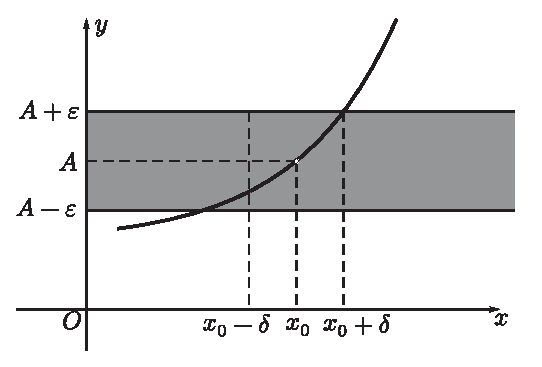
\includegraphics[scale=0.8]{pictures/C-1/极限1.eps}
	\end{center}
	\sj \sj 
	\caption{极限的定义图解}
\end{figure}
\sj
\subsection{自变量趋于无穷大时函数的极限}
\tdefination[函数极限2]
设函数$f(x)$在当$|x|$大于某一正数时恒有定义.如果存在常数$A$,对于任意给定的正数$\varepsilon$(不论它多么小),总存在正数$X$使得当$x$满足不等式$|x|>X$时,对应的函数值$f(x)$都满足不等式
\begin{equation}
|f(x)-A|<\varepsilon
\end{equation}
那么常数$A$就叫做函数$f(x)$当$x \to x_0$的\dy[极限]{JX},记作
\begin{equation}
\lim\limits_{x\to \infty}f(x)=A \huo f(x)\to A(x \to \infty )
\end{equation}

\subsection{无穷小与无穷大}
\tdefination[无穷小]
如果函数$f(x)$当$x\to x_0\left(\mbox{或}x \to \infty  \right) $时的极限为$0$,那么称函数$f(x)$为当$x\to x_0\left(\mbox{或}x \to \infty  \right) $时的\dy[无穷小]{WQX}.记为
\begin{equation}
\lim\limits_{x \to x_0}f(x)=0,\lim\limits_{x\to \infty}f(x)=0.
\end{equation}
特别地,以$0$为极限的数列${x_n}$称为$n\to \infty$时的\dy[无穷小]{WQX}.
\jg

\defination[无穷大]
设函数$f(x)$在$x_0$的某一去心邻域内有定义(或$|x|$趋于某一正数时有定义).如果对于任意给定的正数$M$(不论它多么大),总存在正数$\delta$(或正数$X$),只要$x$适合不等式$0<|x-x_0|<\delta$(或$|x|>X$),对应函数值$f(x)$总满足不等式
\begin{equation*}
|f(x)|>M
\end{equation*}
那么称函数$f(x)$为当$x\to x_0\left(\mbox{或}x \to \infty  \right) $时的\dy[无穷大]{WQD}.记为
\begin{equation}
\lim\limits_{x \to x_0}f(x)=\infty,\lim\limits_{x\to \infty}f(x)=\infty.
\end{equation}

\subsection{单侧极限}
\tdefination[左极限]
在 $\lim\limits_{x \to x_0}f(x)=A$的定义中,把$0<|x-x_0 |<\delta$改为$x_0-\delta <x<x_0$ ,那么$A$就叫做函数$f(x)$当$x \to x_0$时的\dy[左极限]{ZJX}.记作
\begin{equation}
\lim\limits_{x \to x_0^-}f(x)=A \huo f(x_0^-)=A \huo \lim\limits_{x \to x_0 - 0}f(x)=A
\end{equation}

\defination[右极限]
在 $\lim\limits_{x \to x_0}f(x)=A$的定义中,把$0<|x-x_0 |<\delta$改为$x_0 <x<x_0+\delta$ ,那么$A$就叫做函数$f(x)$当$x \to x_0$时的\dy[右极限]{YJX}.记作
\begin{equation}
\lim\limits_{x \to x_0^+}f(x)=A \huo f(x_0^+)=A \huo \lim\limits_{x \to x_0 + 0}f(x)=A
\end{equation}

\subsection{利用定义求函数的极限的解题方法}
\texample[可以直接求得$\delta$与$\varepsilon$的关系]
任意一个$\varepsilon$满足$|f(x)-A|<\varepsilon$,都能找到一个正数$\delta$使$0 < |x - x_0| < \delta$或$|x| > \delta$ ,这就说明了$\varepsilon$与$\delta $有个对应关系,即
\begin{equation}
\delta=\varphi(\varepsilon)
\end{equation}
\par $\delta=\varphi(\varepsilon)$这个关于$\varepsilon$的函数可以是任意的.所以我们利用极限的定义来证明某个函数的极限时,只需找到$\varepsilon$和$\delta$之间的对应关系.这时,我们可以先利用$|f(x)-A|<\varepsilon$这个条件,然后构造出 $|x - x_0| < \varphi(\varepsilon)$的形式即可.(对于求数列的极限时$\delta$换成$N$即可.)

\examples 证明下列极限\\[0.5em]
\hspace*{0.8em} $1.\,\,\lim\limits_{x \to 3}2x-1=5$

\proof  设$\exists \delta,\forall \varepsilon$,当$0<|x-3|<\delta $时,$|2x-1-5|=|2x-6|=2|x-3|<\varepsilon$\quad \quad 【构造$|x-x_0 | < \varphi (\varepsilon)$】\\[0.5em]
即$\displaystyle |x-3|<\frac{\varepsilon}{2}$,故取$\displaystyle \delta = \frac{\varepsilon}{2}$时成立,证毕.\\[1.5em]
\hspace*{0.8em} $2.\,\,\displaystyle \lim\limits_{x \to \infty }\frac{1}{x}=0$\\[1em]
\proof  设$\exists N,\forall \varepsilon$,当$|x|>N$时,$\displaystyle \left| \frac{1}{x}-0\right| =\left| \frac{1}{x}\right|<\varepsilon$\hspace{13em}【构造$|x-x_0 | < \varphi (\varepsilon)$】\\[0.5em]
即$\displaystyle |x|>\frac{1}{\varepsilon}$,故取$\displaystyle N = \frac{1}{\varepsilon}$时成立,证毕.\\

\example[不能直接求得$\delta$与$\varepsilon$的关系]
\noindent 【方法一】放缩法\vspace{0.8em}
\par 这个时候我们可以将$|f (x) - A|$进行适当的放大,使得$\delta $与$\varepsilon$的关系容易求得,一般的放缩方法有:\\[0.5em]
\noindent (1)  将分母恒大于零的部分(可以含$x$)删去;\\[0.5em]
\noindent (2)  将分子恒小于零的部分删去(可以含$x$);\\[0.5em]
\noindent (3)  将幂函数的底数部分进行放缩.

\examples 证明$\displaystyle \lim\limits_{x \to 1}\sqrt{3x+1}=2.$

\proof 设$\exists \delta,\forall \varepsilon$,当$0<|x-1|<\delta $时,$\displaystyle |\sqrt{3x+1}-2|=\frac{3(x-1)}{\sqrt{3x+1}+2}\le \frac{3}{2}|x-1|<\varepsilon$\hspace{4em}【放缩构造】\\[0.5em]
即$\displaystyle |x-1|<\frac{2}{3}\varepsilon$,又$\displaystyle \sqrt{3x+1}$定义域为$\displaystyle x>-\frac{1}{3}$,那么$\displaystyle x-1>-\frac{4}{3}$,在一定范围内有$\displaystyle |x-1|<\frac{4}{3}$\hspace{1em}【判断定义域】\\[0.5em]
故取$\displaystyle \delta = \min \left\lbrace  \frac{2}{3}\varepsilon,\frac{4}{3} \right\rbrace $时成立,证毕.\hspace{27em}【取最小值】\\

\noindent 【方法二】先设后求再取值法\vspace{0.8em}
\par 放缩不是唯一的方法,我们还可以先设后求再取$\delta $最小值.\\[0.5em]
\noindent (1)  先化简式子,且含$|x-a|$项,这个时候可以用该方法;\\[0.5em]
\noindent (2)  设$\delta $的值为$f(a)$ (可以含$a,x$,也可以是常数);\\[0.5em]
\noindent (3)  解出$x$的范围,对非$|x - a|$的项进行放缩,将式子放大,同时使得非$|x - a|$的项转换为常量;\\[0.5em]
\noindent (4)  反解出$\delta = \varphi (\varepsilon)$;\\[0.5em]
\noindent (5)  取$\delta = \min \lbrace f(a),\varphi(\varepsilon)\rbrace$.\vspace{0.5em}
\par 当然通常放缩法和先设后求再取值法会结合用,这样就可以解决大部分题目.\vspace{0.5em}
\par 但是在后面的证明过程中,一般简单的函数极限可以直接用,所以一般情况下不会用定义证明极限.

\examples 证明$\lim\limits_{x \to a}x^2=a^2$

\proof 由于$|x^2-a^2|=|(x-a)(x+a)|=|x-a|\cdot |x+a| $,\hspace{15em}【找到$|x-a|$项】\\[0.5em]
设$\displaystyle |x-a|<\frac{1}{2}$,则$\displaystyle |x+a|=|x-a+2a|\le |x-a|+|2a|<\frac{1}{2}+|2a|.$【赋值$|x-a|$项,并放缩得出未知项的范围】\\[0.5em]
所以,设$\exists \delta,\forall \varepsilon$,当$0<|x-1|<\delta $时,$\displaystyle |x^2-a^2|=|x-a|\cdot |x+a|<\left( \frac{1}{2}+|2a|\right)|x-a|<\varepsilon $,\\[0.5em]
即$\displaystyle|x-a|<\frac{\varepsilon}{\frac{1}{2}+2|a|}$.\hspace{28em}【反解出$|x-a|$的范围】\\[0.5em]
故取$\displaystyle \delta = \min \left\lbrace  \frac{\varepsilon}{\frac{1}{2}+2|a|},\frac{1}{2} \right\rbrace $时成立,证毕.\hspace{24.5em}【取最小值】\\

\subsection{证明函数的极限不存在的方法}
\ttheorem[序列极限]
设函数$f (x)$在$a$点的一个空心邻域内有定义,并且$\lim\limits_{x \to a}f(x)=l$.假若是一串在该空心邻域内取值的序列,且
\begin{equation*}
\lim\limits_{n \to \infty}x_n=a
\end{equation*}
则有
\begin{equation}
\lim\limits_{n \to \infty}f(x_n)=l
\end{equation}
\par 这个定理为我们提供了一种\textbf{证明函数极限不存在的办法}:对于一个定义在$a$点的某空心邻域内的函数$f(x)$,如果能找到两串序列$\lbrace x'_n \rbrace $与$\lbrace x''_n\rbrace$它们都在$a$的该空心邻域内取值,且当$n\to \infty $时都以$a$为极限,而极限$\lim\limits_{n \to \infty }x'_n$与 $\lim\limits_{n \to \infty }x''_n$都存在但不相等,则$f(x)$在$x \to a$时不可能有极限.\jg

\example[证明函数的极限不存在]
\sj \examples 证明:函数$\displaystyle \sin \frac{1}{x}$在$x\to 0$时没有极限.

\proof 取$\displaystyle x'_n=\frac{1}{2n\pi }$,则$\displaystyle \sin \frac{1}{x'_n}=0$;而取$\displaystyle x''_n=\frac{1}{2n\pi+\frac{\pi}{2} }$,则$\displaystyle \sin \frac{1}{x'_n}=1.$\\[0.5em]
这时由于$n \to \infty \Rightarrow x'_n\to 0,x''_n \to 0, $且
\begin{equation*}
\lim\limits_{n \to \infty} \sin \frac{1}{x'_n} \ne \lim\limits_{n \to \infty} \sin \frac{1}{x''_n} 
\end{equation*}
因此,函数$\displaystyle \sin \frac{1}{x}$在$x\to 0$时没有极限.

\section{利用极限运算法则和两个准则求极限}
\subsection{极限运算法则}
\ttheorem[极限运算法则1]
两个无穷小的和是无穷小.

\tl 有限个无穷小的和是无穷小.
\newpage
\theorem[极限运算法则2]
有界函数与无穷小的乘积是无穷小.

\tl 常数与无穷小的乘积是无穷小.

\tl 有限个无穷小的乘积是无穷小.\jg

\theorem[极限运算法则3]
如果$\lim f(x) = A, \lim g(x) = B$(这些函数都必须存在极限),那么
\begin{equation}
\lim [f(x)\pm g(x)]=\lim f(x)\pm \lim g(x)=A \pm B
\end{equation}
\begin{equation}
\lim[f(x)\cdot g(x)]=\lim f(x)\cdot \lim g(x)=A\cdot B
\end{equation}
若$B\ne 0$,那么
\begin{equation}
\lim \left[ \frac{f(x)}{g(x)}\right] =\frac{\lim f(x)}{\lim g(x)}=\frac{A}{B}
\end{equation}

\tl 如果$\lim f(x)$存在,而$c$为常数,那么
\begin{equation}
\lim [cf(x)]=c \lim f(x)
\end{equation}

\tl 如果$\lim f(x)$存在而$n$为正整数,那么
\begin{equation}
\lim [f(x)]^n=[\lim f(x)]^n
\end{equation}

\theorem[极限运算法则4]
如果$\varphi(x) \ge \psi(x),$而$\lim \varphi(x)=A,\lim \psi(x)=B,$则$A \ge B.$\jg

\subsection{极限运算准则}
\ttheorem[单调有界数列极限一定存在]
(1)  \quad 若$x_{n+1} \le x_n(n\mbox{为正整数})$,且$x_n \ge m,$则$\lim\limits_{n \to \infty }x_n = A $存在,且$A \ge m$;\jg
\par (2)  \quad 若$x_{n+1} \ge x_n(n\mbox{为正整数})$,且$x_n \le M,$则$\lim\limits_{n \to \infty }x_n = A $存在,且$A \le M$.

\theorem[夹逼定理]
设$g(x) \le f(x) \le h(x)$,若$\lim\limits_{x \to m}g(x)=A,\lim\limits_{x \to m}=A,(-\infty \le m \le +\infty)$则$\lim\limits_{x \to m}f(x)=A.$\jg

\subsection{例题}
\texample[利用极限运算法则和两个准则求极限]\sj
\examples 证明:$\lim\limits_{n \to \infty}q^n=0.(|q|<1)$

\proof 设$\displaystyle |q|=\frac{1}{1+a},a>0,$则$\displaystyle 0< q^n=\frac{1}{(1+a)^n}=\frac{1}{C^0_na^0=C^1_na^1+C^2_na^2+\cdots+C^n_na^n}<\frac{1}{C^1_na^1}=\frac{1}{na}.$\\[0.5em]
又$\displaystyle \lim\limits_{n \to \infty}\frac{1}{na}=0,\lim\limits_{n\to \infty}0=0,$由夹逼定理可得
\begin{equation*}
\lim\limits_{n\to \infty}0 \le \lim\limits_{n \to \infty}q^n \le \lim\limits_{n \to \infty}\frac{1}{na}
\end{equation*}
故$\lim\limits_{n \to \infty}q^n=0.$\jg

\examples 证明:$\displaystyle a_n=\frac{a^n}{n!}(a\mbox{是大于1的任意常数})$存在极限.

\proof 当$n>[a]+1$时,有
\begin{equation*}
0\le a_n =\frac{a^{[a]}}{[a]!}\cdot \frac{a}{[a]+1}\cdot \frac{a}{[a]+2}\cdot \,\,\cdots \,\,\cdot \frac{a}{n}<\frac{a^{[a]}}{[a]!}\cdot \frac{a}{n}
\end{equation*}
注意到$\displaystyle \frac{a^{[a]}}{[a]!}$是一个常数,所以$\displaystyle \lim\limits_{n \to \infty}\frac{a^{[a]}}{[a]!}\cdot \frac{a}{n}=0,$由夹逼定理可得
\begin{equation*}
\lim\limits_{n \to \infty}a_n=0.
\end{equation*}

\examples 设常数$a>1,$对于任意自然数$k$,证明:
\begin{equation*}
\lim\limits_{n \to \infty}\frac{n^k}{a^n}=0.
\end{equation*}
\hspace*{-0.5em}\proof 令$t=a-1$,则$t>0$,那么
$$a_n=(1+t)^n=1+nt+\frac{n(n-1)}{2!}t^2+\cdots+\frac{n(n-1)\cdot(n-k)}{(k+1)!}t^{k+1}+\cdots+t^n,$$
因此,当$n>1$时,$\displaystyle a^n>\frac{n(n-1)\cdots(n-k)}{(k+1)!}t^{k+1}$,于是
$$
0 \le \frac{n^k}{a^n}\le \frac{n^k}{\displaystyle \frac{n(n-1)\cdots(n-k)}{(k+1)!}t^{k+1}}=\frac{(k+1)!}{t^{k+1}}\cdot \frac{n^k}{n(n-1)\cdots(n-k)}=\frac{(k+1)!}{t^{k+1}}\cdot\frac{n^k}{\lambda_{k+1}n^{k+1}+\lambda_kn^k+\cdots+\lambda_1n+\lambda_0}
$$
其中$\lambda_0,\lambda_1,\cdots,\lambda_{k+1}$均为非零常数.注意到$\displaystyle \frac{(k+1)!}{t^{k+1}}$为常数,则
\begin{equation*}
\begin{split}
&\quad \, \lim\limits_{n \to \infty}\frac{(k+1)!}{t^{k+1}}\cdot\frac{n^k}{\lambda_{k+1}n^{k+1}+\lambda_kn^k+\cdots+\lambda_1n+\lambda_0}\\
&=\lim\limits_{n \to \infty}\frac{(k+1)!}{t^{k+1}}\cdot\frac{1}{n}\cdot \frac{n^k}{\lambda_{k+1}+\lambda_kn^{-1}+\cdots+\lambda_1n^{-k}+\lambda_0n^{-k-1}}=0
\end{split}
\end{equation*}
因此,由夹逼定理可得
\begin{equation*}
\lim\limits_{n \to \infty}\frac{n^k}{a^n}=0.
\end{equation*}

\section{利用等价无穷小求极限}
\subsection{无穷小的分类}
\tdefination[无穷小的分类]
设$\alpha,\beta $是同一变化过程中的无穷小,$\displaystyle \lim \frac{\beta}{\alpha}$是这一过程的极限,$c$为常数,那么\\[0.5em]
\noindent (1) \quad $\displaystyle \lim \frac{\beta }{\alpha}=0$,则称$\beta $是$\alpha $的\dy[高阶无穷小]{GJWQX},记作$\beta = o(\alpha)$.\\[0.5em]
\noindent (2) \quad  $\displaystyle \lim \frac{\beta }{\alpha}=\infty$,则称$\beta $是$\alpha $的\dy[低阶无穷小]{DJWQX1}.\\[0.5em]
\noindent (3) \quad  $\displaystyle \lim \frac{\beta }{\alpha}=c \ne 0$,则称$\beta $是$\alpha $的\dy[同阶无穷小]{TJWQX}.\\[0.5em]
\noindent (4) \quad  $\displaystyle \lim \frac{\beta }{\alpha}=1$,则称$\beta $是$\alpha $的\dy[等价无穷小]{DJWQX2},记作$\beta \sim \alpha$.\\[0.5em]
\noindent (3) \quad  $\displaystyle \lim \frac{\beta }{\alpha^k}=c \ne 0$,则称$\beta $是$\alpha $的\dy[$k$阶无穷小]{KJWQX}.\\[0.5em]
\color{black}{{\CJKfamily{heiti}注意}}\quad 0与``0"的区别\\[0.5em]
\noindent (i)\quad ``0"指的是无穷小,设$\alpha$是某一变化过程中的无穷小,也就是说$x$趋于某一值时,极限为0.\\[0.5em]
\noindent (ii)\quad 当0指的是实数0时,$\lim 0 \cdot f(x)=0$,这与$f(x)$无关,即使$\lim f(x)=\infty$,其结果仍然是0,因为0在这里时实数,而不是无穷小.\jg

\subsection{常见的等价无穷小}
\ttheorem[常见的等价无穷小]
以下等价无穷小均为$x \to 0$这一变化过程,其中$x$也可替换为一个函数,即$f(x) \to 0$的情况也适用.
\begin{equation}
\tan x \sim \sin x \sim x \sim \arcsin x \sim \arctan x
\end{equation}
\begin{equation}
\ln (1+x) \sim x
\end{equation}
\begin{equation}
x \sim \e^x -1
\end{equation}
\begin{equation}
1-\cos x \sim \frac{x^2}{2}
\end{equation}
\begin{equation}
\sec x -1 =\frac{1}{\cos x}-1 \sim \frac{x^2}{2}
\end{equation}
\begin{equation}
(1+x)^a-1 \sim 1-ax
\end{equation}
\begin{equation}
a^x-1 \sim \ln a \cdot x \,(a>0,a \ne 1)
\end{equation}
\subsection{等价无穷小求极限的本质}
等价无穷小求极限本质上是极限与1的相乘,而有等价无穷小的定义,1可以换成极限$\displaystyle 1=\lim\limits_{x \to x_0}\frac{\alpha }{\beta}$,再运用极限乘法运算法则计算即可.

\example[等价无穷小的误用]\sj
\examples 求极限$\displaystyle \lim\limits_{x \to 0}\frac{\tan x -\sin x}{\sin^3 x}$.

\errsolve  由于$\tan \sim \sin x \sim x$得$\displaystyle \lim\limits_{x \to 0}\frac{\tan x -\sin x}{\sin^3 x}=\lim\limits_{x \to 0}\frac{x-x}{\sin^3 x}=\lim\limits_{x \to 0}0=0.$

\errreason  在运用等价无穷小的时候没有考虑极限运算法则成立的条件.

\solvereason $\displaystyle \lim\limits_{x \to 0}\frac{\tan x -\sin x}{\sin^3 x}=\lim\limits_{x \to 0}\frac{\tan x}{\sin^3 x} - \lim\limits_{x \to 0}\frac{\sin x}{\sin^3 x}$实际上运用了法则$\lim [f(x)-g(x)]=\lim f(x)-\lim g(x),$\\[1em]即完整的错解解题步骤应为
\begin{equation*}
\lim\limits_{x \to 0}\frac{\tan x -\sin x}{\sin^3 x}=\lim\limits_{x \to 0}\frac{\tan x}{\sin^3 x} - \lim\limits_{x \to 0}\frac{\sin x}{\sin^3 x}
=\lim\limits_{x \to 0}\frac{\tan x}{\sin^3 x}\cdot \lim\limits_{x \to 0} \frac{x}{\tan x}-\lim\limits_{x \to 0}\frac{x}{\sin^3 x}
\end{equation*}
而极限运算法则成立的条件是$\lim f(x),\lim g(x)$存在,而$\displaystyle \lim\limits_{x \to 0}\frac{\tan x}{\sin^3 x}$不存在,因此解题错误.

\solve $\displaystyle \lim\limits_{x \to 0}\frac{\tan x -\sin x}{\sin^3 x}=\lim\limits_{x \to 0}\frac{\sin x(\sec x-1)}{\sin^3 x}=\lim\limits_{x \to 0}\frac{\sec x-1}{\sin^2 x} \cdot \lim\limits_{x \to 0}\frac{\frac{x^2}{2}}{\sec x -1} \cdot \lim\limits_{x \to 0}\frac{\sin x^2}{x^2}
=\frac{\frac{x^2}{2}}{x^2}=\frac{1}{2}.$



